\documentclass[preprint,12pt]{elsarticle}
% \documentclass[draft,12pt]{elsarticle}

\usepackage{hyperref}
\usepackage{graphicx}
\usepackage{subcaption}
\usepackage{amssymb}
\usepackage{amsmath}
\usepackage{multirow}
\usepackage{relsize}
\usepackage[utf8]{inputenc}
\usepackage{cleveref}
\usepackage{algorithm}
\usepackage[noend]{algpseudocode}
\usepackage[section]{placeins}
\usepackage{booktabs}
\usepackage{url}

% For the TODOs
\usepackage{xcolor}
\usepackage{xargs}
\usepackage[colorinlistoftodos,textsize=footnotesize]{todonotes}
\newcommand{\todoin}{\todo[inline]}
% from here: https://tex.stackexchange.com/questions/9796/how-to-add-todo-notes
\newcommandx{\unsure}[2][1=]{\todo[linecolor=red,backgroundcolor=red!25,bordercolor=red,#1]{#2}}
\newcommandx{\change}[2][1=]{\todo[linecolor=blue,backgroundcolor=blue!25,bordercolor=blue,#1]{#2}}
\newcommandx{\info}[2][1=]{\todo[linecolor=OliveGreen,backgroundcolor=OliveGreen!25,bordercolor=OliveGreen,#1]{#2}}

%Boldtype for greek symbols
\newcommand{\teng}[1]{\ensuremath{\boldsymbol{#1}}}
\newcommand{\ten}[1]{\ensuremath{\mathbf{#1}}}

\usepackage{lineno}
% \linenumbers

\journal{}

\begin{document}

\begin{frontmatter}

  \title{Study of mixing behaviour of spherical particles in fluid using stirrer}
  \author[XXX]{Dinesh Adepu\corref{cor1}}
  \ead{d.dinesh@surrey.ac.uk}
  \author[University of Surrey]{Chuan Yu Wu}
  \ead{XXX}
\address[xxx]{xxx}

\cortext[cor1]{Corresponding author}


\begin{abstract}
  Particle dispersion is a fundamental physical phenomenon encountered in
  various industries where powder and fluid interactions are
  pivotal. Particularly, processes involving the mixing of powder with fluid
  using a stirrer are commonplace. While experimental investigation of such
  processes is often impractical due to their highly nonlinear nature,
  numerical methods offer a viable alternative. Among these, Smoothed Particle
  Hydrodynamics coupled with Discrete Element Method (SPH-DEM) stands out for
  its ability to handle free surface fluid dynamics and model the complex
  physics inherent in dispersion processes.


  In this study, we initially develop and validate both the DEM and SPH
  solvers. Validation includes testing against fundamental benchmarks such as
  two-particle head-on collisions and particle-wall impacts for the DEM
  solver, and Poiseuille flow for the fluid solver. Additionally, we validate
  the rigid-fluid model through simulations of a single cylindrical body
  entering a steady tank and the settling of two tandem cylinders in a
  fluid-filled tank.


  With confidence in the fidelity of our solver established, we delve into
  investigating the mixing behavior of spherical particles dispersed in
  water. Our study encompasses various scenarios, including particles with
  densities higher or lower than the surrounding fluid, as well as particles
  with varying radii. We also examine combinations of these factors.
  \todoin{What factor have you considered to quantify the mixing
    behaviour.}

  \todoin{Write the findings}
\end{abstract}

\begin{keyword}
%% keywords here, in the form: keyword \sep keyword
{xxx}, {xxx}, {xxx}

%% MSC codes here, in the form: \MSC code \sep code
%% or \MSC[2008] code \sep code (2000 is the default)

\end{keyword}

\end{frontmatter}

% \linenumbers


\FloatBarrier%
\section{Introduction}

\begin{figure}[!htpb]
  \centering
  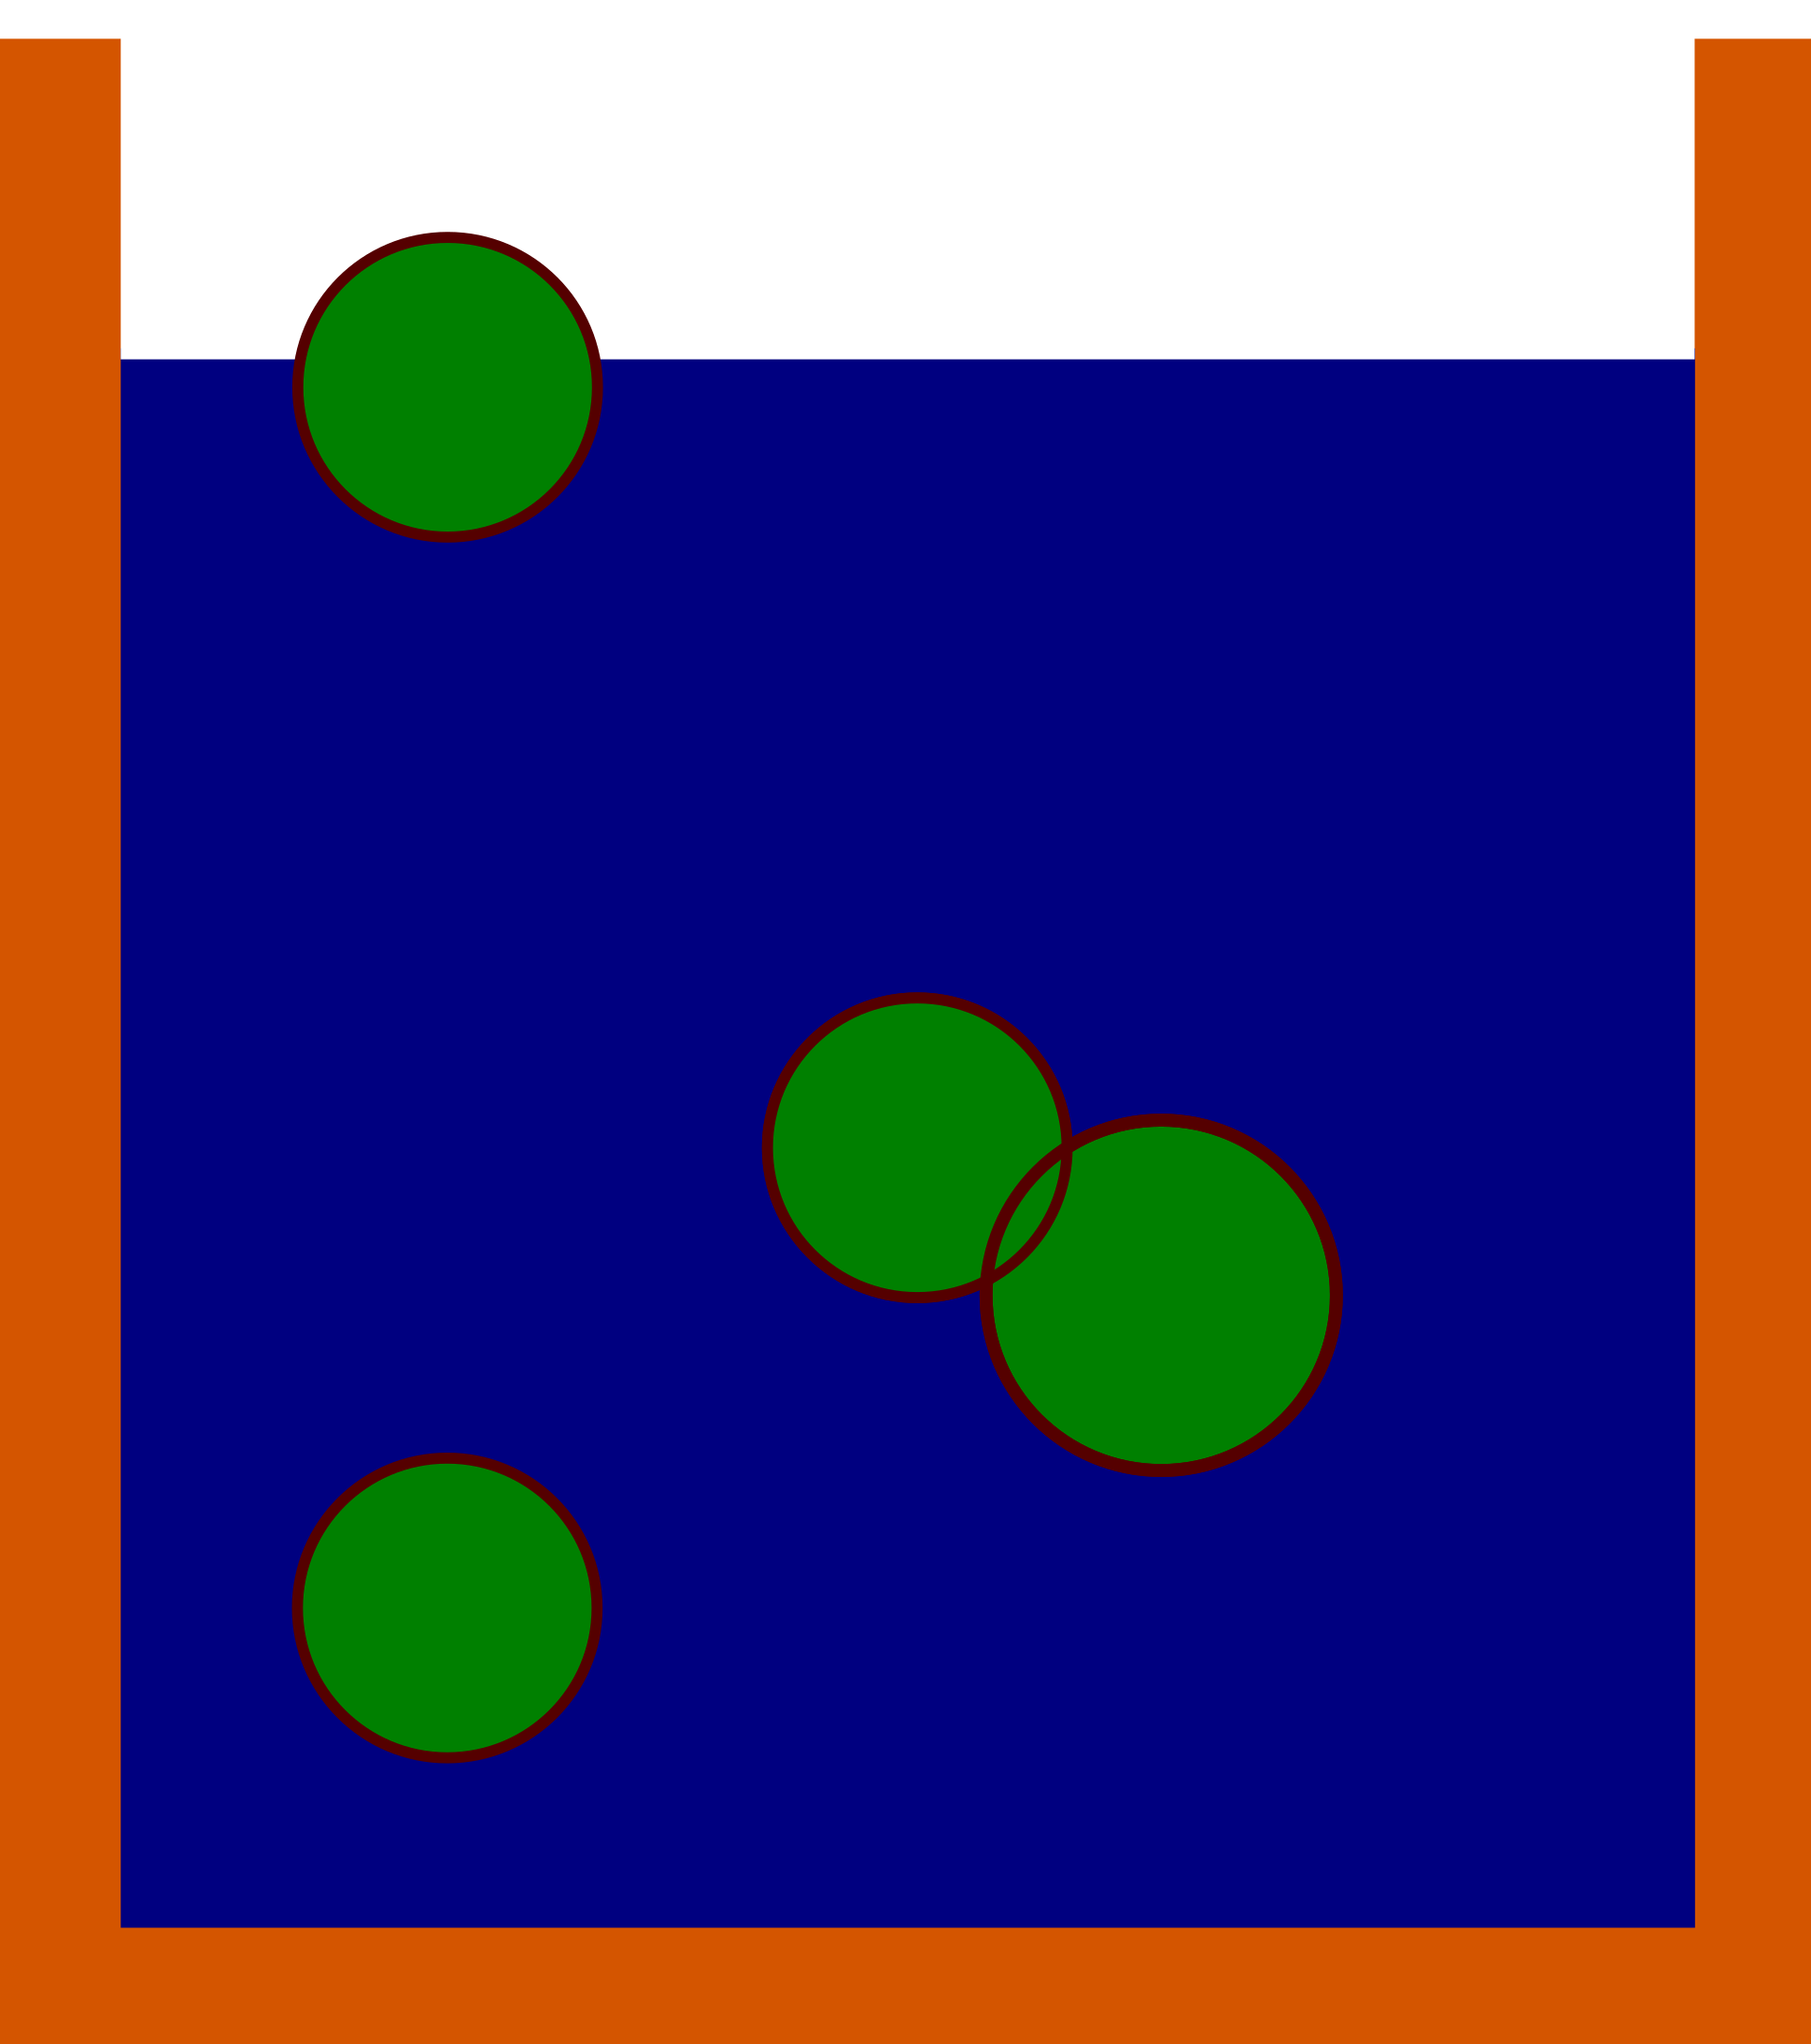
\includegraphics[width=0.4\textwidth]{images/hs_tank_fluid_with_particles}
  \caption{Body frame and local frame description of rigid body}
  \label{fig:gloabl_body_frame_rb}
\end{figure}

\begin{itemize}
\item Fluid modeling using smoothed particle hydrodynamics
  (\cref{sec:fluid--modeling})
\item Interaction among the discrete spherical rigid particle units by
  discrete element method (\cref{sec:rbd})
\end{itemize}

While the interaction among the rigid spherical particle and fluid particles
are modeled by sampling the spherical particles into dummy SPH particles. This
is explained in \cref{sec:rfc}.





% \FloatBarrier%
% \section{Fluid modeling}


% \FloatBarrier%
% \subsection{Boundary conditions}



% \FloatBarrier%
% \section{Solid phase modeling}


% \FloatBarrier%
% \subsection{Discrete element method}


% \FloatBarrier%
% \subsection{Rigid body equations}


% \FloatBarrier%
% \section{Rigid fluid coupling}


% \FloatBarrier%
% \section{Results}



\FloatBarrier%
\subsection{Fluid modeling}
\label{sec:fluid--modeling}

In the current work, we follow a weakly-compressible SPH approach to model the
fluid. The SPH discretization of the continuity
equation~\cref{eq:sph-discretization-continuity} and the momentum equation
~\cref{eq:sph-momentum-fluid} respectively are,
\begin{equation}
  \label{eq:sph-discretization-continuity}
  \frac{{d}\rho_a}{dt} = \sum_{b} \; \frac{m_b}{\rho_{b}} \;
  \rho_{a} \; {\ten{u}}_{ab} \; \cdot \nabla_{a} W_{ab},
\end{equation}

%
Similarly, the discretized momentum equation for fluids is written as,
\begin{multline}
  \label{eq:sph-momentum-fluid}
  \frac{{d}\ten{u}_{a}}{dt} = - \sum_{b} m_b
  \bigg(\frac{p_a}{\rho_a^2} + \frac{p_b}{\rho_b^2}\bigg)
  \nabla_{a} W_{ab}
 \;+\;
  \sum_{b} m_b \frac{4 \eta \nabla W_{ab}\cdot
    \ten{r}_{ab}}{(\rho_a + \rho_b) (r_{ab}^2 + 0.01 h_{ab}^2)} \ten{u}_{ab}  \;+\;
  \ten{g}_{a} + \text{force due to rb},
\end{multline}
where $\ten{I}$ is the identity matrix, $\eta$ is the kinematic viscosity of the
% fluid and \textcite{morris1997modeling} formulation is used to discretize the
viscosity term.

We add to the momentum equation an additional artificial viscosity term
% $\Pi_{ab}$~\parencite{monaghan-review:2005} to maintain the stability of the
numerical scheme, given as,
\begin{align}
  \label{eq:mom-av}
  \Pi_{ab} =
  \begin{cases}
\frac{-\alpha h_{ab} \bar{c}_{ab} \phi_{ab}}{\bar{\rho}_{ab}}
  & \ten{u}_{ab}\cdot \ten{r}_{ab} < 0, \\
  0 & \ten{u}_{ab}\cdot \ten{r}_{ab} \ge 0,
\end{cases}
\end{align}
where,
%
\begin{equation}
  \label{eq:av-phiij}
  \phi_{ab} = \frac{\ten{u}_{ab} \cdot \ten{r}_{ab}}{r^2_{ab} + 0.01 h^2_{ab}},
\end{equation}
%
where $\ten{r}_{ab} = \ten{r}_a - \ten{r}_b$,
$\ten{u}_{ab} = \ten{u}_a - \ten{u}_b$, $h_{ab} = (h_a + h_b)/2$,
$\bar{\rho}_{ab} = (\rho_a + \rho_b)/2$, $\bar{c}_{ab} = (c_a + c_b) / 2$, and
$\alpha$ is the artificial viscosity parameter.  The pressure $p_a$ is evaluated
using an equation of state:
\begin{equation}
\label{eqn:sph-eos}
  p_a = K \bigg(\frac{\rho_a}{\rho_{0}} - 1 \bigg).
\end{equation}
Where, $K=\rho_0 \, c_0^2$ is bulk modulus of the body, with
$c_0=10 \times V_{\text{max}}$ is speed of sound, while $\rho_0$ as the
initial density of the particles.


\FloatBarrier%
\subsection{Boundary conditions}
\label{sec:boundary_conditions}


\FloatBarrier%
\section{Rigid body dynamics}
\label{sec:rbd}
% The rigid body is discretized into particles with equal spacing each particle
% with mass $m_i$ and density $\rho_i$. Rigid body has a total 6 degrees of
% freedom (DOF), divided into $3$ translational and $3$ rotational.
The equations governing the dynamics of a rigid body are, balance of linear and
angular momentum given by,
\begin{equation}
  \label{eq:rfc:balance_linear_mom}
  \frac{d \; (M \ten{v}_{cm})}{d t} = \sum_i \ten{F}_i,
\end{equation}
\begin{equation}
  \label{eq:rfc:balance_angular_mom}
  \frac{d \ten{L}}{d t} = \teng{\tau}_{cm},
\end{equation}
where $M$, $\ten{v}_{cm}$ are the mass and velocity of the center of mass of the rigid body.
$\ten{F}_i, \teng{\tau}_{cm}, \ten{L} $ are force acting at point $i$, torque and
angular momentum about the center of mass of the rigid body. In the current
case, force acting on the particle $i$, $\ten{F}_i$, is due to the interaction
with the other bodies and with the fluid particles, and any other body forces.
The torque $\teng{\tau}_{cm}$ and angular momentum $\ten{L}$ are computed as,
\begin{equation}
  \label{eq:rfc:torque}
 \teng{\tau}_{cm} = \sum_i \ten{F}_i \times (\ten{x}_{cm} - \ten{x}_{i}),
\end{equation}
\begin{equation}
  \label{eq:rfc:moi}
  \teng{L} =
  \sum_i \; \ten{r}_i \times \; (\teng{\omega} \times \ten{r}_i)
  = \sum_i \; m_i \; [(\ten{r}_i \cdot \ten{r}_i) \ten{I} - \ten{r}_i \otimes \ten{r}_i].
\end{equation}
Here $\ten{x}_{cm}$ and $\omega$ are the position of the center of mass and
angular velocity of the rigid body. $m_i$, $\ten{x}_{i}$, $\ten{r}_i$ are the
mass, position of particle, and position of particle $i$ with respect to vector
center of mass.

\begin{figure}[!htpb]
  \centering
  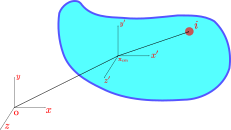
\includegraphics[width=0.7\textwidth]{images/rigid_body/rigid_body}
  \caption{Body frame and local frame description of rigid body}
  \label{fig:gloabl_body_frame_rb}
\end{figure}
We use two coordinate frames to capture the dynamics of the rigid body, a
global frame and a body frame as shown in
\cref{fig:gloabl_body_frame_rb}. The body fixed frame, which moves with
rigid body is always located at the center of mass ($\ten{x}_{cm}$). The
state of the rigid body at a given time ($t$) can be described using position
($\ten{x}_{cm}$) and velocity ($\ten{v}_{cm}$) of the center of mass, a
rotation matrix($\ten{R}$) to represent the orientation of the rigid body with
respect to the global frame, and angular velocity($\teng{\omega}$). The center
of mass is computed as
\begin{equation}
  \label{eq:rfc:center_of_mass}
  \ten{x}_{cm} = \frac{\sum_i m_i \; \ten{x}_{i} }{\sum_i m_i }.
\end{equation}
The position of the discretized particle ($i$) in
\cref{fig:gloabl_body_frame_rb} belonging to the rigid body at time $t$ can be
computed as,
\begin{equation}
  \label{eq:rfc:rb_particle_pos_update}
  \ten{x}_i = \ten{x}_{cm} + \ten{r}_{i},
\end{equation}
with
\begin{equation}
  \label{eq:rfc:rb_particle_pos_update}
  \ten{r}_i = \ten{R} \overline{\ten{r}}_{i}.
\end{equation}
Here $\overline{\ten{r}}_{i}$ is the position of the particle $i$ about the body
frame axis and remains constant through out the simulation. The rotation matrix
$\ten{R}$ is used to bring the body frame position vector to the global frame
$\ten{O}$. Similarly the velocity vector is computed as,
\begin{equation}
  \label{eq:rfc:rb_particle_vel_update}
  \ten{v}_i = \ten{v}_{cm} + \teng{\omega} \times \ten{r}_{i}.
\end{equation}

We evolve the state of the rigid body through the integration of the
\cref{eq:rfc:balance_linear_mom,eq:rfc:balance_angular_mom}. The linear velocity of the
center of mass ($\ten{v}_{cm}$) and angular momentum ($\ten{L}$) at the next
timestep are computed as,
\begin{equation}
  \label{eq:rfc:lin_vel_cm_update}
  \ten{v}_{cm}^{n+1} = \ten{v}_{cm}^{n} + \frac{\ten{F}_{cm}}{M} \; \Delta t,
\end{equation}
\begin{equation}
  \label{eq:rfc:ang_mom_update}
  \ten{L}^{n+1} = \ten{L}^{n} + \teng{\tau}_{cm} \; \Delta t.
\end{equation}
Here, $\ten{F}_{cm} = \sum_i \ten{F}_i$.

The position of the center of mass and the rotation matrix ($\ten{R}$) are updated
by,
\begin{equation}
  \label{eq:rfc:lin_pos_cm_update}
  \ten{x}_{cm}^{n+1} = \ten{x}_{cm}^{n} + \ten{v}_{cm}^{n} \; \Delta t,\\
  \ten{R}^{n+1} = \ten{R}^{n} + \tilde{\teng{\omega}}^{n} \, \ten{R}^{n} \; \Delta t,
\end{equation}
where $\tilde{\teng{\omega}}^{n}$ is matrix formulation of angular velocity
$\omega$. The angular velocity at the new time step is computed with
\begin{equation}
  \label{eq:rfc:ang_velocity_update}
  \teng{\omega}^{n+1} = (\textit{\teng{I}}^{-1})^{n+1} \; \ten{L}^{n+1}.
\end{equation}
Here, moment of inertia at the new time step is computed as,
\begin{equation}
  \label{eq:rfc:moi_update}
  (\textit{\teng{I}}^{-1})^{n+1} = \ten{R}^{n+1} \textit{\teng{\overline{I}}}^{-1} (\ten{R}^{n+1})^T.
\end{equation}
where moment of inertia ($\textit{\teng{\overline{I}}}^{-1}$) in body frame is
used to compute in global frame at every time instant for faster computations.
The moment of inertia ($\textit{\teng{\overline{I}}}$) is computed as,
\begin{equation*}
\textit{\teng{\overline{I}}} =
\begin{bmatrix}
\sum_i m_i (y_i^2 + z_i^2) & -\sum_i m_i x_iy_i & -\sum_i m_i x_iz_i\\
-\sum_i m_i x_iy_i & \sum_i m_i (x_i^2 + z_i^2) &  -\sum_i m_i y_iz_i\\
-\sum_i m_i  x_iz_i & -\sum_i m_i y_iz_i & \sum_i m_i (x_i^2 + y_i^2)
\end{bmatrix}.
\end{equation*}

The position and velocity of the particles of the rigid body are updated by
\begin{eqnarray}
  \label{eq:rfc:rb_particle_pos_update}
  \ten{r}_i = \ten{R} \cdot \overline{\ten{r}}_{i},\\
  \ten{x}_i = \ten{x}_{cm} + \ten{r}_{i},\\
  \ten{v}_i = \ten{v}_{cm} + \teng{\omega} \times \ten{r}_{i}.
\end{eqnarray}

The force acting on particle $i$ is composed of interaction with the other rigid
bodies, and the fluid, given as
\begin{eqnarray}
  \label{eq:rfc:rb_particle_pos_update}
  \ten{F}_i = \ten{F}_{\text{Fl}}^i + \ten{F}_{\text{cont}}^i
\end{eqnarray}
We follow \cref{sec:contact-algorithm} to compute force
$\ten{F}_{\text{cont}}^a$ acting on particle $i$ due to the interaction with
the rigid bodies. The force $\ten{F}_{\text{Fl}}^i$ acting due to the
interaction with the fluid particles follows \cref{subsec:fsi}.



\FloatBarrier%
\subsection{Contact resolution}
\label{sec:dem}

\begin{figure}[!htpb]
  \centering
  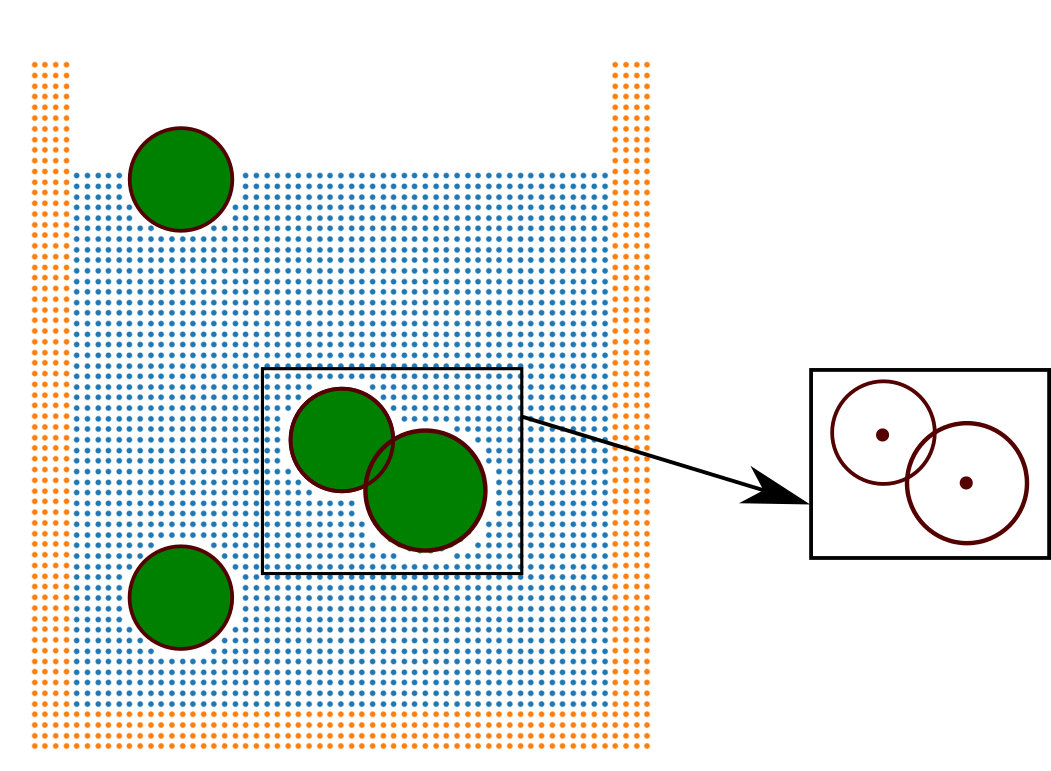
\includegraphics[width=0.7\textwidth]{images/spherical_particles_dem_representation}
  \caption{Body frame and local frame description of rigid body}
  \label{fig:gloabl_body_frame_rb}
\end{figure}

We resolve the contact among the spherical particles using discrete element
method. In the current work we have utilized the contact force model proposed
by \citet{mohseni2021particle}. The force acting on a particle $a$ due to the
interaction with the particle $b$ can be resolved into a normal and tangential
component. The normal force component is utilised to make sure that the
particle do not penetrate into each other, while the tangential component is
used to model the friction between the interacting solids.  The normal force
($\teng{F}_a^{n}$) on particle $a$ due to the interaction with the particles
$b$ is given as,
\begin{equation}
  \label{eq:contact-algorithm-normal}
  \ten{F}_a^n = k_r \delta_{n^{c}}^{a} \ten{n}_a^{c}.
\end{equation}
Here, the overlap $\delta_{n^{c}}^{a}$ is computed using
\begin{equation}
  \label{eq:cf-overlap}
  \delta_{n^{c}}^{a} = \Delta x - d_a,
\end{equation}
where the normal contact vector $\ten{n}_a^{c}$ is computed using
\begin{equation}
  \label{eq:cf-normal-vector}
  \ten{\hat{n}}_a^{c} = \frac{
    \displaystyle\sum\limits_{b = 1}^{\text{NP}^{b}} \;
    \frac{\ten{r}_{ab}}{r_{ab}}  \frac{m_b}{\rho_b} W_{ab}}
  {
    \displaystyle\sum\limits_{b = 1}^{\text{NP}^{b}} \;
    \frac{m_b}{\rho_b} W_{ab}},
\end{equation}
\begin{equation}
  \label{eq:cf-normal-vector}
  \ten{n}_a^{c} = \frac{\teng{\hat{n}}_a^{c}}{||\teng{\hat{n}}_a^{c}||}.
\end{equation}
With $\Delta x$ being the initial spacing between the particles, $k_r$ is the normal
spring stiffness coefficient. Note that while computing the overlap of
particle $a$ with the body $B$ we have computed an effective overlap, rather
than per particle interaction. This effectively is able to model the
interaction between non smooth surfaces in contrast with particle-particle
force computation.


\subsection{Tangential force computation}
\label{sec:tangential-force-computation}
We associate a tangential spring attached to particle $i$ and body $B$ to
compute the tangential force, which initially has a magnitude of zero
($|\Delta \textit{\textbf{l}}_a|=0$). And the tangential spring is activated
when the particle comes into contact with body $B$. The tangential force is
history-dependent. The contact friction force is proportional to the
tangential spring displacement, which is integrated over the contact time as
\begin{equation}
  \label{eq:tangential-force}
  \ten{F}_{a}^{t^{n+1}} =
  -k_f \Delta \textit{\textbf{l}}_a^{\,n + 1} =
  -k_f \big[\big(\Delta {\textit{\textbf{l}}}_a^{\,n} \
  + \ten{v}_{ab}^{n + 1} \Delta t\big) \cdot \ten{t}_a^{n + 1} \big] \
  \ten{t}_a^{n + 1},
\end{equation}
where $\Delta t$ is the time step, $\ten{v}_{ab} = \ten{v}_{a} - \ten{v}_b$ is
the relative velocity of the primary particle $a$ with respect to the
closest secondary particle $b$, and $k_f$ is the tangential spring stiffness
coefficient. The tangential unit vector is computed by,
\begin{equation}
  \label{eq:tangential-vect}
  \ten{t}_a = \frac{\ten{v}_{ab} - (\ten{v}_{ab} \cdot \ten{n}_a^{c}) \ten{n}_a^{c}}{|\ten{v}_{ab} - (\ten{v}_{ab} \cdot \ten{n}_a^{c}) \ten{n}_a^{c}|}.
\end{equation}

The tangential force is coupled to the normal force through the Coulomb's law,
\begin{equation}
  \label{eq:Coulomb-law}
  \ten{F}_{a}^{t} = \min(\mu |\ten{F}_{a}^{n}|, |\ten{F}_{a}^{t}|) \
  \frac{\ten{F}_{a}^{t}}{|\ten{F}_{a}^{t}|}.
\end{equation}
This allows us to impose the sliding friction condition between the
interacting solids. Finally, the total force acting on the particle $a$ due to
the interaction with body $B$ is:
\begin{equation}
  \label{eq:contact-force}
  \ten{F}_{a}^{\text{cont}} = \ten{F}_{a}^{n} + \ten{F}_{a}^{t}
\end{equation}

% \begin{figure}[!htpb]
%   \centering
%   \includegraphics[width=0.3\textwidth]{images/contact_force/contact_force_description_3}
%   \caption{Force transfer to the secondary particles $b$ from the primary body particle $a$}
% \label{fig:secondary_particle_contact_foce_transfer}
% \end{figure}
An equal and opposite force of the same magnitude is applied to the closest
secondary particle $b$ of $a$ as shown in
\cref{fig:secondary_particle_contact_foce_transfer},
\begin{equation}
  \label{eq:contact-force}
  \ten{F}_{b}^{\text{cont}} = - \ten{F}_{a}^{\text{cont}}.
\end{equation}


% =========================================== %
% ------ Results start ---------------------- %
% =========================================== %


\FloatBarrier%
\subsection{Rigid fluid coupling}
\label{sec:rfc}

\begin{figure}[!htpb]
  \centering
  \begin{subfigure}{0.22\textwidth}
    \centering
    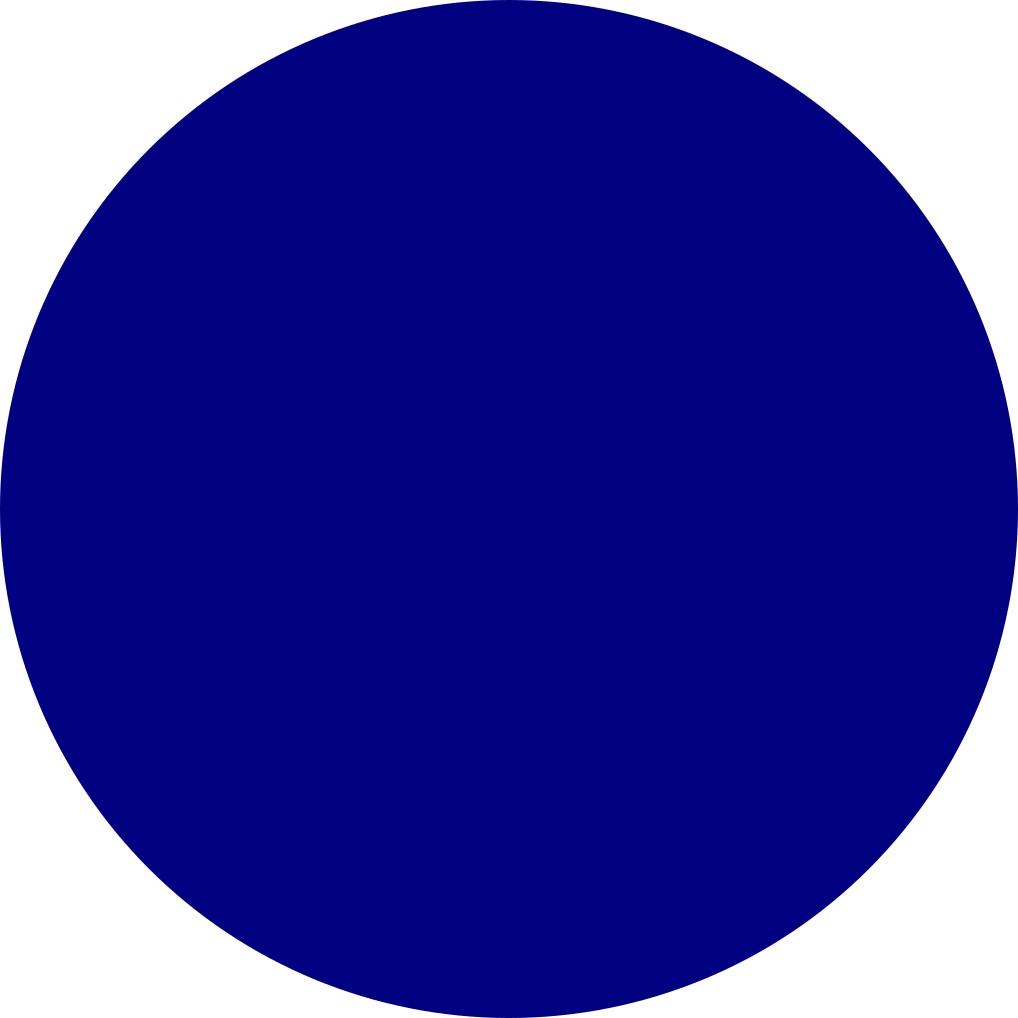
\includegraphics[width=1.0\textwidth]{images/rfc_explantion_schematic/real_spherical_particles}
    \subcaption{}%\label{fig:rings:ipst-nu-0.47-0}
  \end{subfigure}\hspace{15mm}%
  \begin{subfigure}{0.24\textwidth}
    \centering
    
\includegraphics[width=1.0\textwidth]{images/rfc_explantion_schematic/sph_sampled_spherical_particles}
    \subcaption{}%\label{fig:rings:ipst-nu-0.47-1}
  \end{subfigure}
  \caption{}
\label{fig:real_particle_sph_sampling}
\end{figure}
In order to compute the force acting on the spherical particle due to the
interacting fluid we sample the spherical particle with dummy SPH particles,
as shown in \cref{fig:real_particle_sph_sampling}. Here the spherical particle
is sampled using dummy SPH particles, while SPH particles are being placed
equispaced. With spherical particles being discretized into SPH particles and
immersed in fluid can be seen in \cref{fig:many_rb_in_fluid_sph_particles}.
\begin{figure}[!htpb]
  \centering
  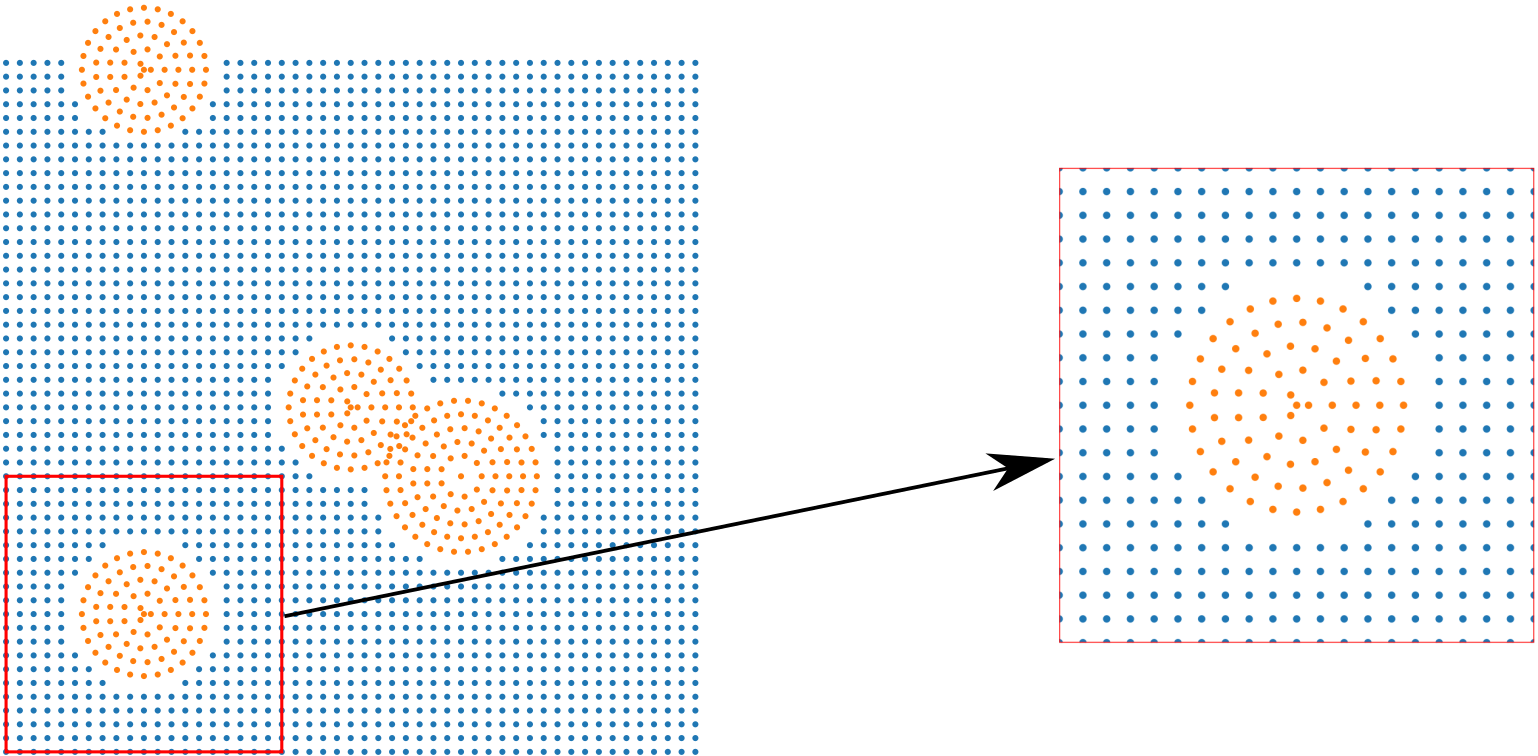
\includegraphics[width=0.7\textwidth]{images/rfc_zoomed_combined}
  \caption{Body frame and local frame description of rigid body}
  \label{fig:many_rb_in_fluid_sph_particles}
\end{figure}


Force on each sampled SPH particles consisting of the rigid body due to the
interaction with the fluid particle is given as. The mass of each dummy
particle being sampled in the spherical particle is considered as
hydrodynamics mass. The force on the fluid particle due to the interaction
with the sampled dummy SPH particles is considered in the momentum and the
continuity equation. The force acting on the sampled dummy SPH particle due to
the interaction with the fluid is given by,
\begin{equation}
  \label{eq:sph-discretization-continuity}
  \frac{{d}\rho_a}{dt} = \sum_{b} \; \frac{m_b}{\rho_{b}} \;
  \rho_{a} \; {\ten{u}}_{ab} \; \cdot \nabla_{a} W_{ab},
\end{equation}
The force here is composed of two components, one is due to the pressure and
due to viscosity.



\FloatBarrier%
\subsection{Time Integration}

Rigid body and the fluid follow the kick-drift-kick time integration scheme. The
modeling of rigid-rigid interaction requires lower time step than the fluid. We
choose the minimum of both the timesteps to move the system forward in time. For
the numerical stability of fluid, the time step depends on the CFL condition as,
\begin{equation}
  \label{eq:rfc:time-step-cfl}
  \Delta t_{\text{fluid}} = \mathrm{min} \bigg( 0.25 \; \frac{h}{c + |U|} ,  0.25 \; \frac{h^2}{\nu},  0.25 \; \frac{h^2}{g} \bigg),
\end{equation}
where $|U|$ is the maximum velocity magnitude, $c$ is the speed of sound
typically chosen as $10 |U|$ for fluids in this work. For rigid body, the time
step is constrained as,
\begin{equation}
  \label{eq:rfc:time-step-body-force}
  \Delta t_{\text{rb}} \leq \frac{\pi}{50} \sqrt{\frac{m}{K_r}}.
\end{equation}
A minimum timestep is chosen as
\begin{equation}
  \label{eq:rfc:time-step-body-force}
  \Delta t = min(\Delta t_{\text{fluid}}, \Delta t_{\text{rb}}).
\end{equation}



\FloatBarrier%
\section{Results}
\label{sec:results}



\FloatBarrier%
\subsection{Poiseuille's flow}
\label{sec:poiseuille_flow}
% https://onlinelibrary.wiley.com/doi/epdf/10.1002/nag.898

\begin{itemize}
\item Unsteady flow between two infinite, parallel paltes at rest in presence
  of pressure gradient.
\item Write about the location of the plates.
\item Which way the flow is going (positive x or negative x)
\item In this exact conditions, the Navier-Stokes equations admit the time
  dependent solution (Write solution (equation 19))
\item Periodic boundary conditions
\item The accuracy of the results presented here validate the developed
  no-slip boundary method inthe presence of straight boundaries.  The
  remainder of this section addresses the more complexcase of non-straight
  boundaries.
\item Write about the schematic
\item Write the resulting velocity profile
\item Numerical parameters are important
\item A body force of 1e-5
\item Viscosity 0.01
\item Time of 50 seconds
\item spacing of 1 / 60
\item Length in y is 2 * self.d=0.5
\item Length in x 0.4 * self.Ly
\item self.re = self.options.re
\item self.Vmax = self.nu*self.re/(2*self.d)
\item self.c0 = 10*self.Vmax
\item self.p0 = self.c0**2*self.rho0
\item self.fx = self.Vmax * 2*self.nu/(self.d**2)
\end{itemize}

The analytical solution from Morris is given as


\begin{equation}
  \label{eq:sph-discretization-continuity}
  v_x(y, t) = \frac{F}{2 \nu}y(y - L) + \sum_{n=0}^{\infty}\frac{4FL^2}{\nu \pi^3 (2n + 1)^3} \sin\bigg(\frac{\pi y}{L} (2 n + 1) \bigg) \exp\bigg(\frac{ (2 n + 1)^2 \pi^2 \nu}{L^2} t\bigg)
\end{equation}

$\nu$ is kinematic viscosity ($\frac{\mu}{\rho_0}$)


\begin{figure}[!htpb]
  \centering
  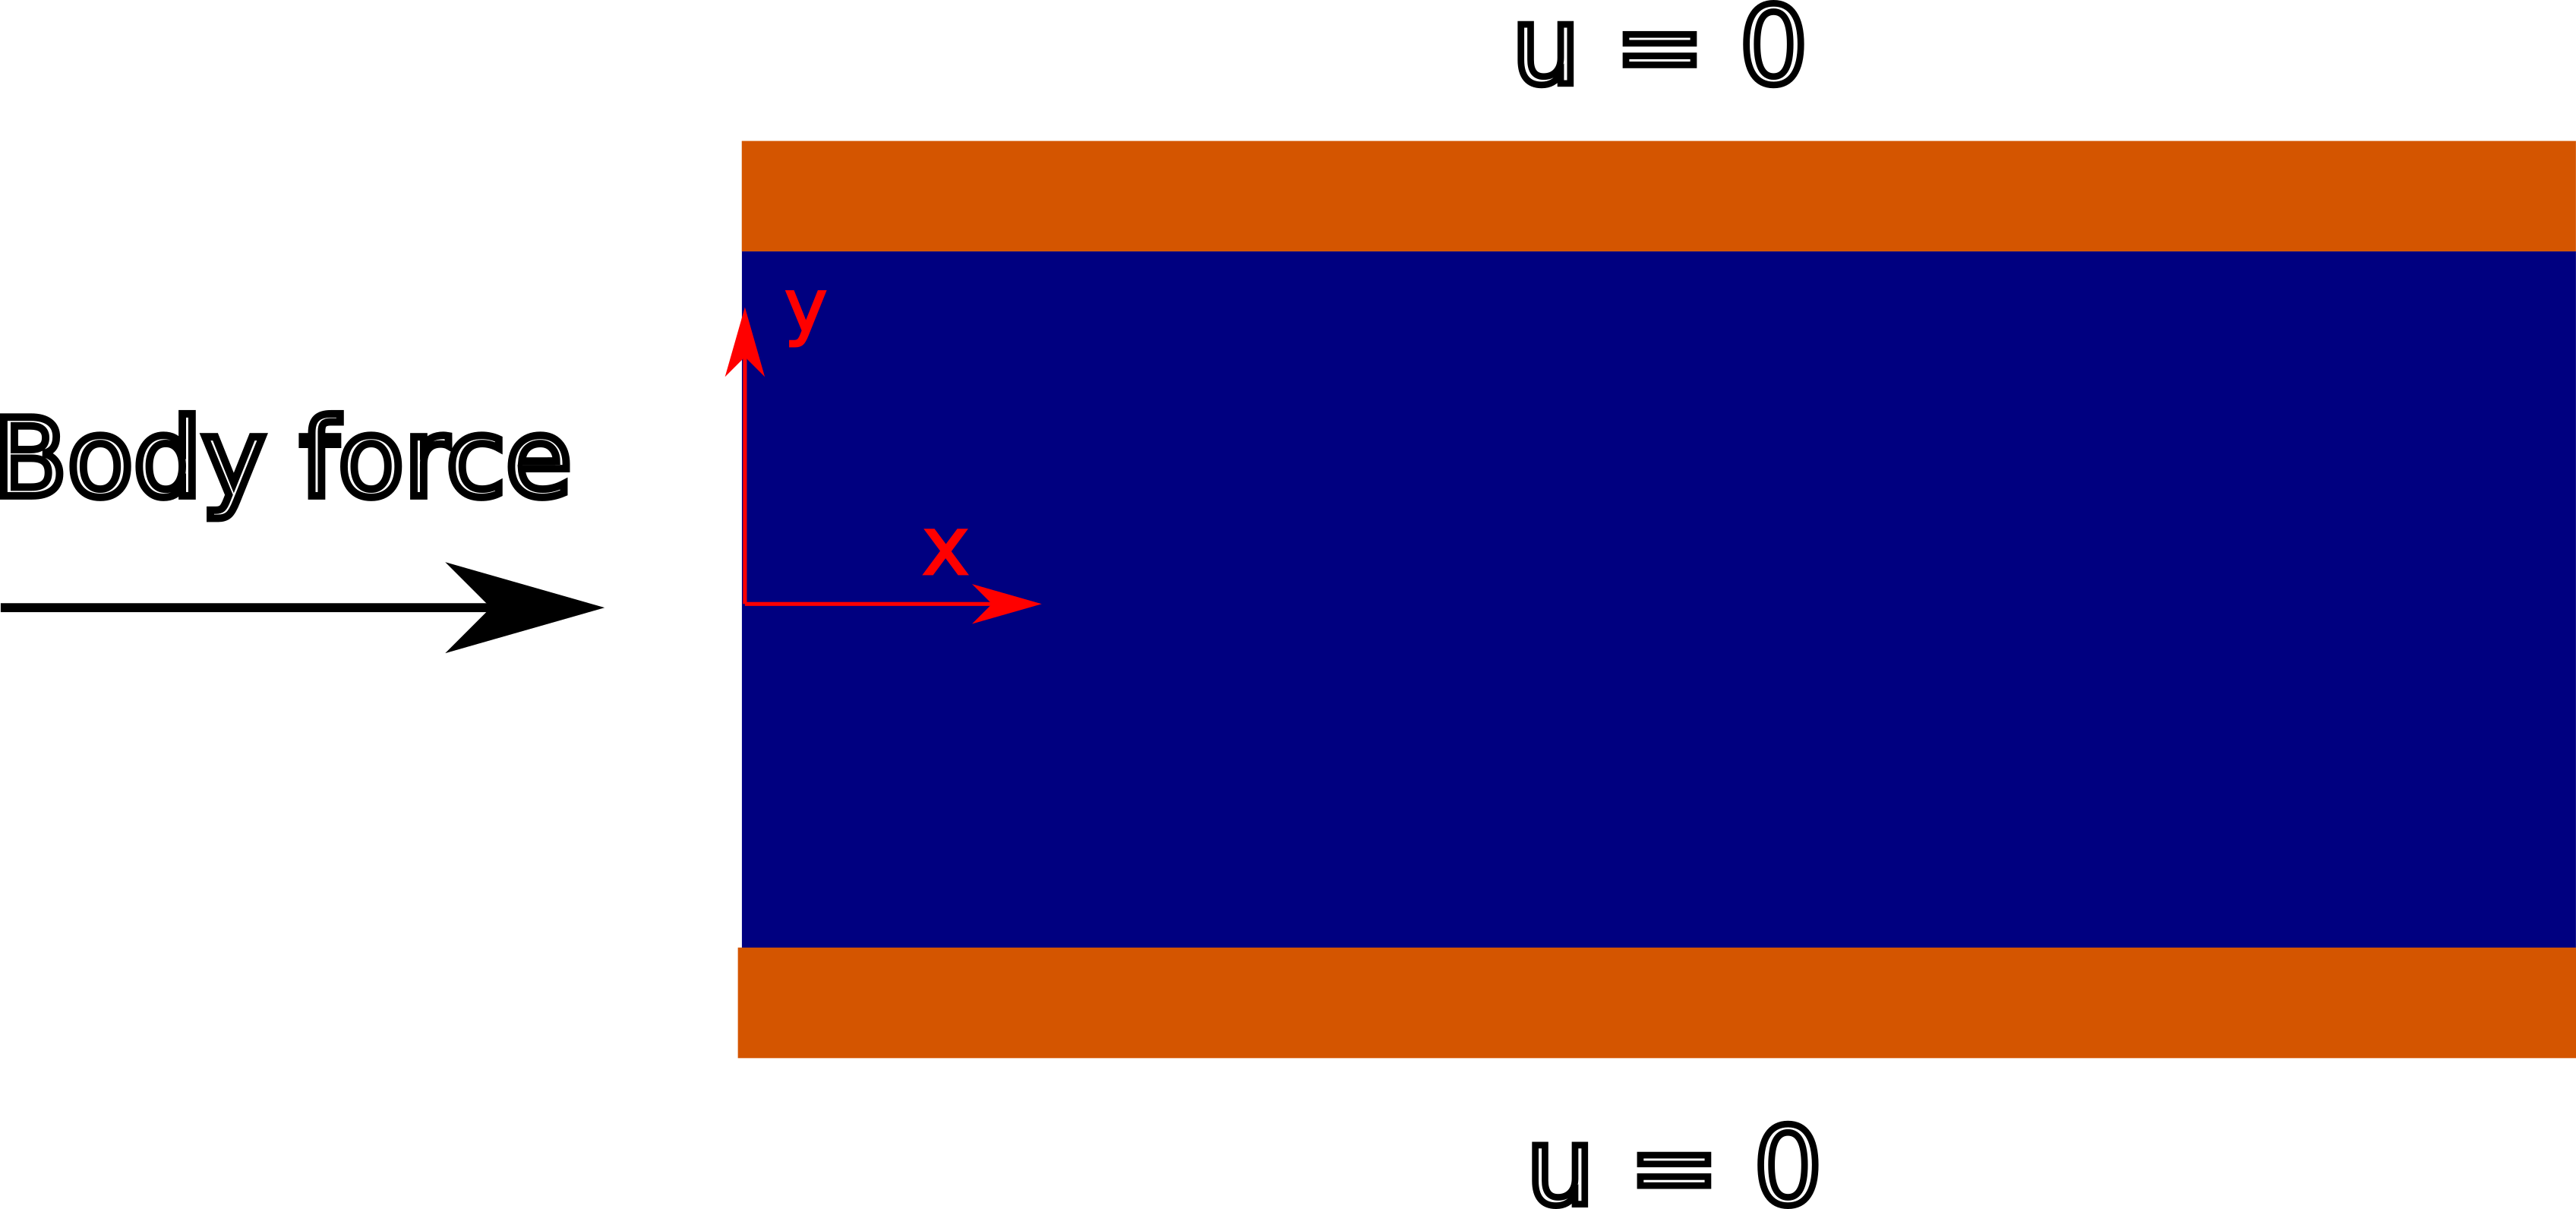
\includegraphics[width=0.4\textwidth]{images/fluid_01_benchmark_poisuelle/poiseuille_schematic}
  \caption{Body frame and local frame description of rigid body}
  \label{fig:gloabl_body_frame_rb}
\end{figure}

\begin{figure}[!htpb]
  \centering
  \includegraphics[width=0.4\textwidth]{figures/plane_poiseuille_flow_2D/case_1/comparison.png}
  \caption{Body frame and local frame description of rigid body}
  \label{fig:gloabl_body_frame_rb}
\end{figure}


\FloatBarrier%
\subsection{DEM validation 1: Normal impact of spherical particle}
\label{sec:DEM_validation_1_normal_impact}

\begin{figure}[!htpb]
  \centering
  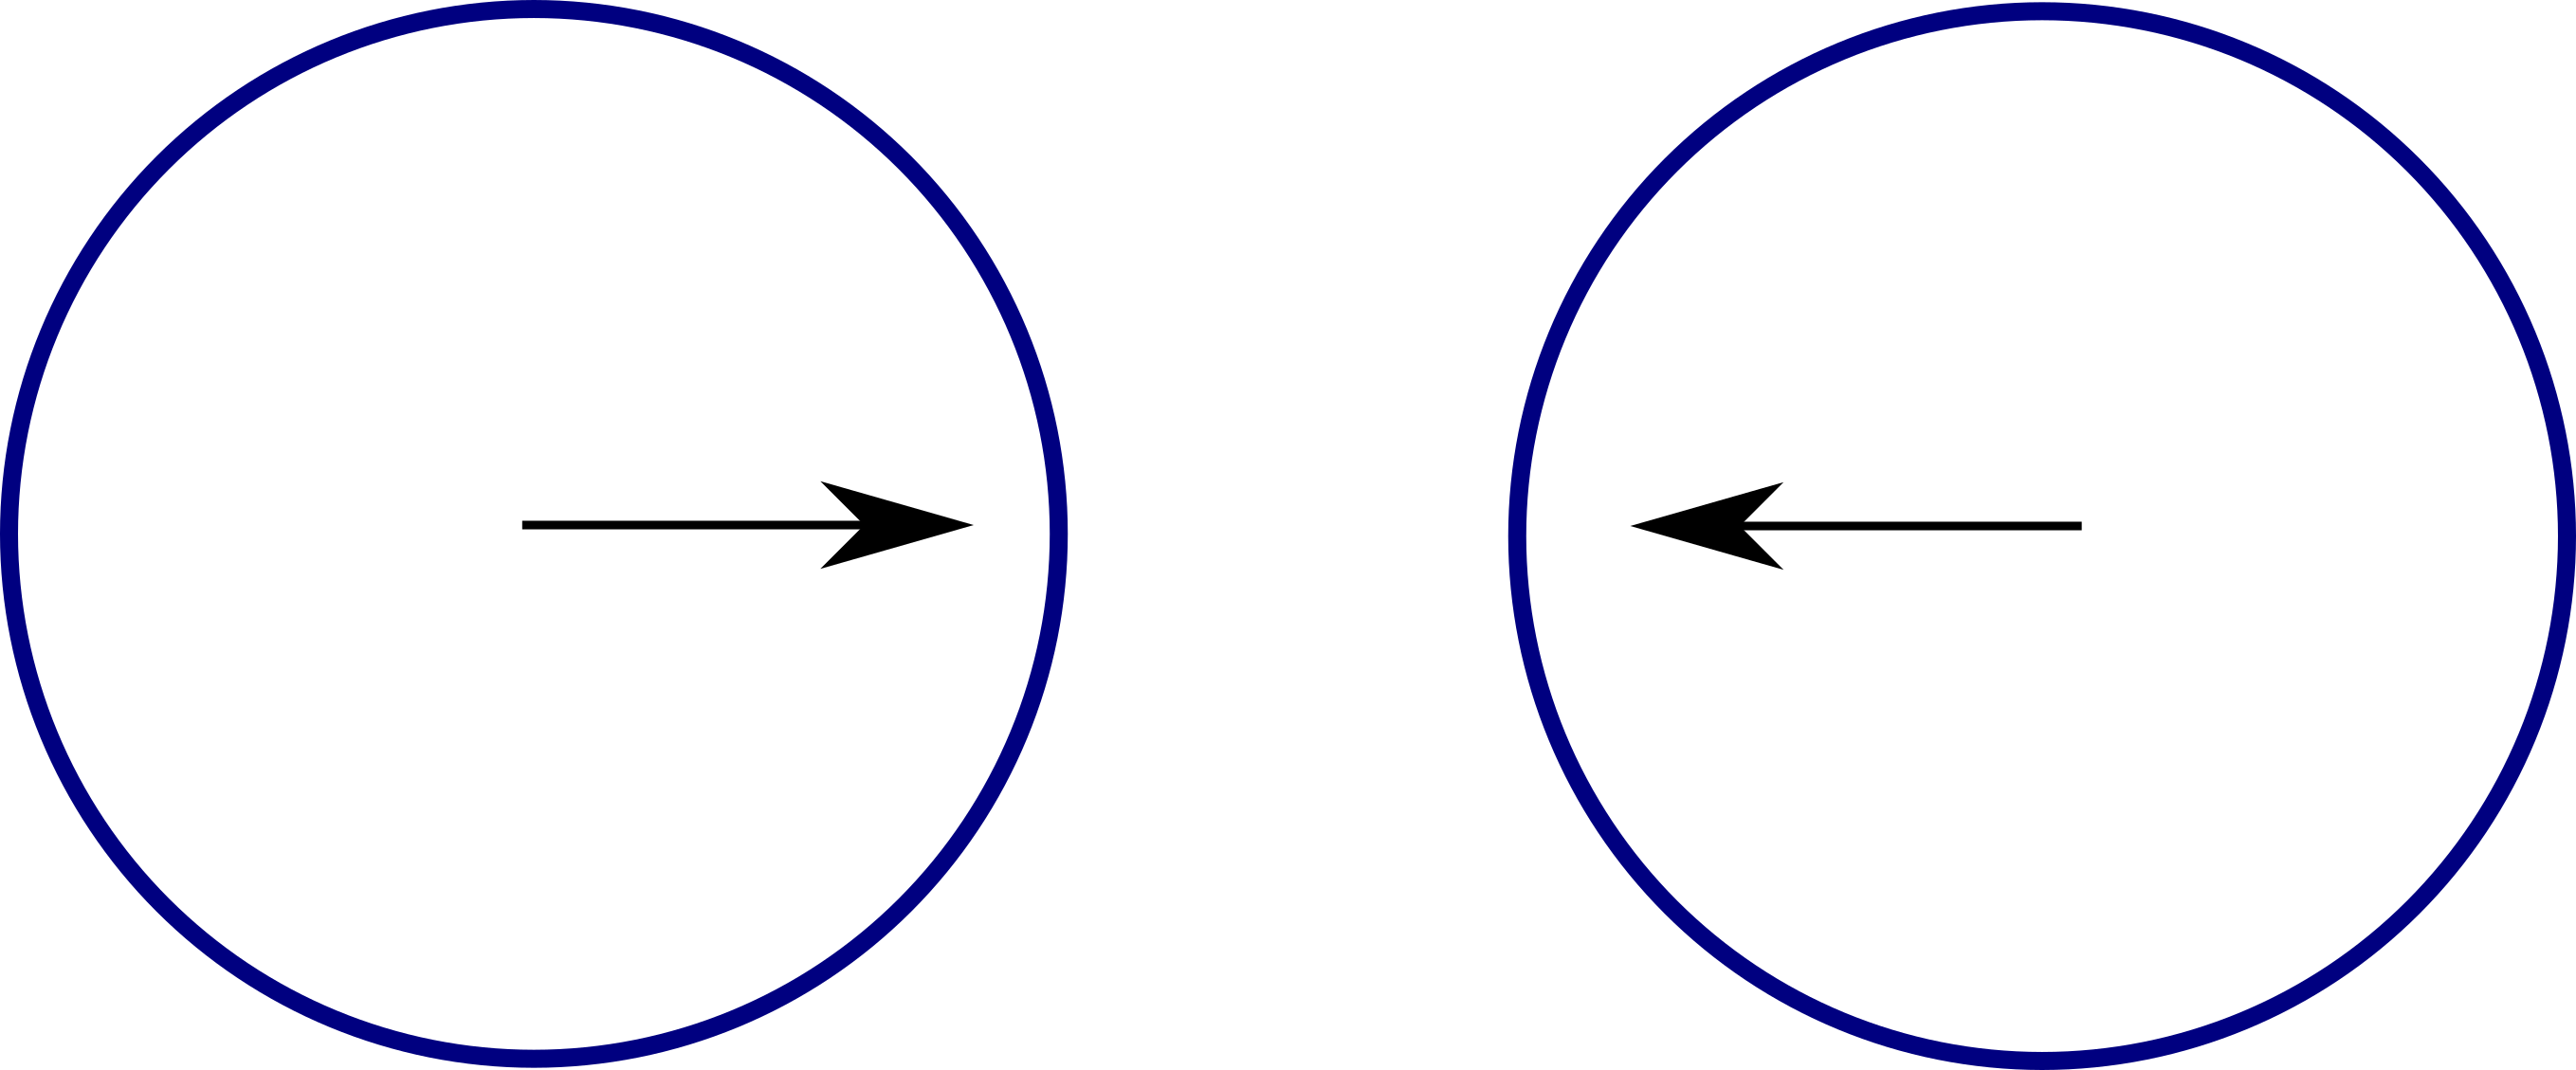
\includegraphics[width=0.4\textwidth]{images/results_dem_1_validation_particle_particle_impact/dem_01_head_on_schematic}
  \caption{Body frame and local frame description of rigid body}
  \label{fig:result:dem_1_schematic}
\end{figure}
For the initial validation of the Discrete Element Method (DEM), we examine
the head-on collision of two spherical particles. In
\cref{fig:result:dem_1_schematic}, the initial setup depicts both particles
moving towards each other with an initial velocity of $10$
m\,s\textsuperscript{-1}.  Each disk has a radius of $0.01$ m and is composed
of glass. The glass material has a Young's modulus of $4.8 \times 10^{10}$
N\,m\textsuperscript{-2}, a Poisson ratio of $0.2$, and a density of $2800$
kg\,m\textsuperscript{-3}.  For the current scenario, we assume there is no
friction or gravity acting on the particles.
\Cref{fig:result:dem_1_force_vs_overlap} depicts the variation of the normal
force and the amount of overlap, compared to the analytical findings presented
in \citet{xxxx}. The force curve generated by our current implementation
closely matches the analytical result, confirming the validation of our DEM
solver's normal contact force model.
\begin{figure}[!htpb]
  \centering
  \includegraphics[width=0.4\textwidth]{figures/benchmark_1_ss_colliding_elastic/fn_vs_overlap}
  \caption{Body frame and local frame description of rigid body}
  \label{fig:result:dem_1_force_vs_overlap}
\end{figure}


\FloatBarrier%
\subsection{DEM validation 2: Particle wall impact}
\label{sec:DEM_validation_2_particle_wall_impact}
\begin{figure}[!htpb]
  \centering
  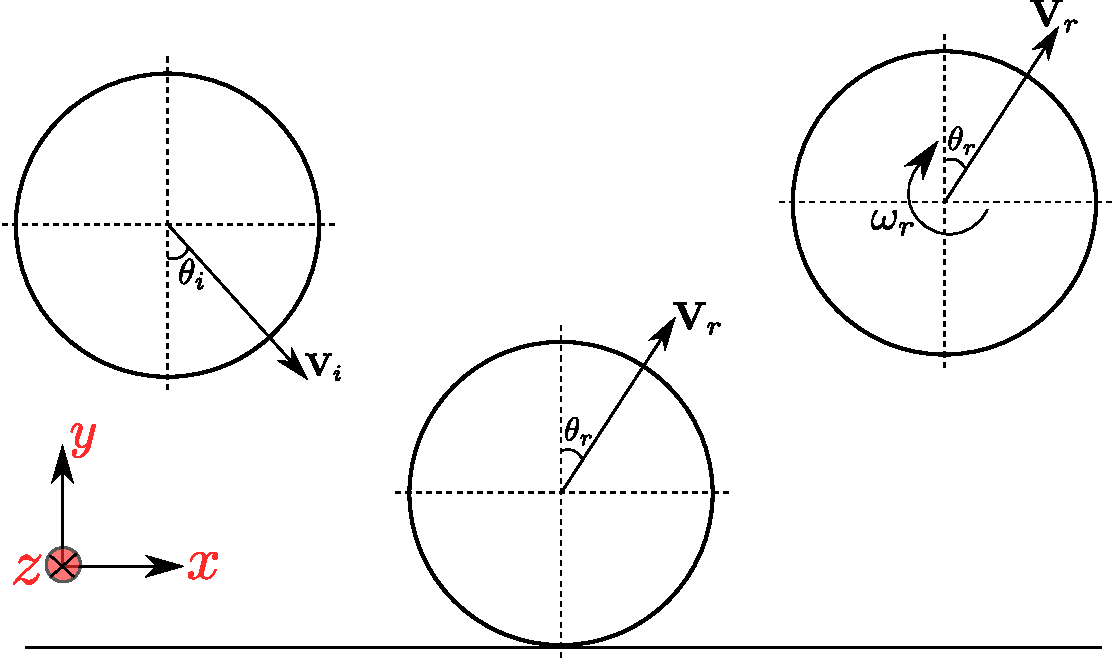
\includegraphics[width=0.4\textwidth]{images/results_dem_2_validation_particle_wall_impact/schematic}
  \caption{}
  \label{fig:result:dem_sw_contact_schematic}
\end{figure}
As part of our validation test cases, we consider the collision of a spherical
particle with wall with different incident angles and a constant velocity in
magnitude. This test case is helpful in testing the tangential part of our DEM
implementation. The schematic of the body and wall is shown in
\cref{fig:result:dem_sw_contact_schematic}. The radius of the impacting particle is
$0.0025$ m and is made of aluminium oxide. The particle has a Young's modulus
of $3.8 \times 10^{11}$ N\,m\textsuperscript{-2}, a Poisson ratio of $0.23$, and a
density of $4000$ kg\,m\textsuperscript{-3}. The impact velocity has a
magnitude of $3.9$ m\,s\textsuperscript{-1}. The friction coefficient among
the wall and the particle is $0.092$.


In \cref{fig:result:dem_sw_contact_omega_vs_theta}, we plot the variation of
the rebound angular velocity with the incident impact angle, compared against
the experimental result given in \citet{xxxx}. The variation of the angular
velocity produced by our current implementation matches with the experimental
result, confirming the validation of our DEM solver's tangential part of the
contact force model.
\begin{figure}[!htpb]
  \centering
  \includegraphics[width=0.4\textwidth]{figures/benchmark_4_sw_colliding_oblique/angle_vs_ang_vel.pdf}
  \caption{Body frame and local frame description of rigid body}
  \label{fig:result:dem_sw_contact_omega_vs_theta}
\end{figure}


\FloatBarrier%
\subsection{RFC validation 1: Single particle entering into a tank}
\label{sec:rfc_validation_1_single_particle_entry}
\begin{figure}[!htpb]
  \centering
  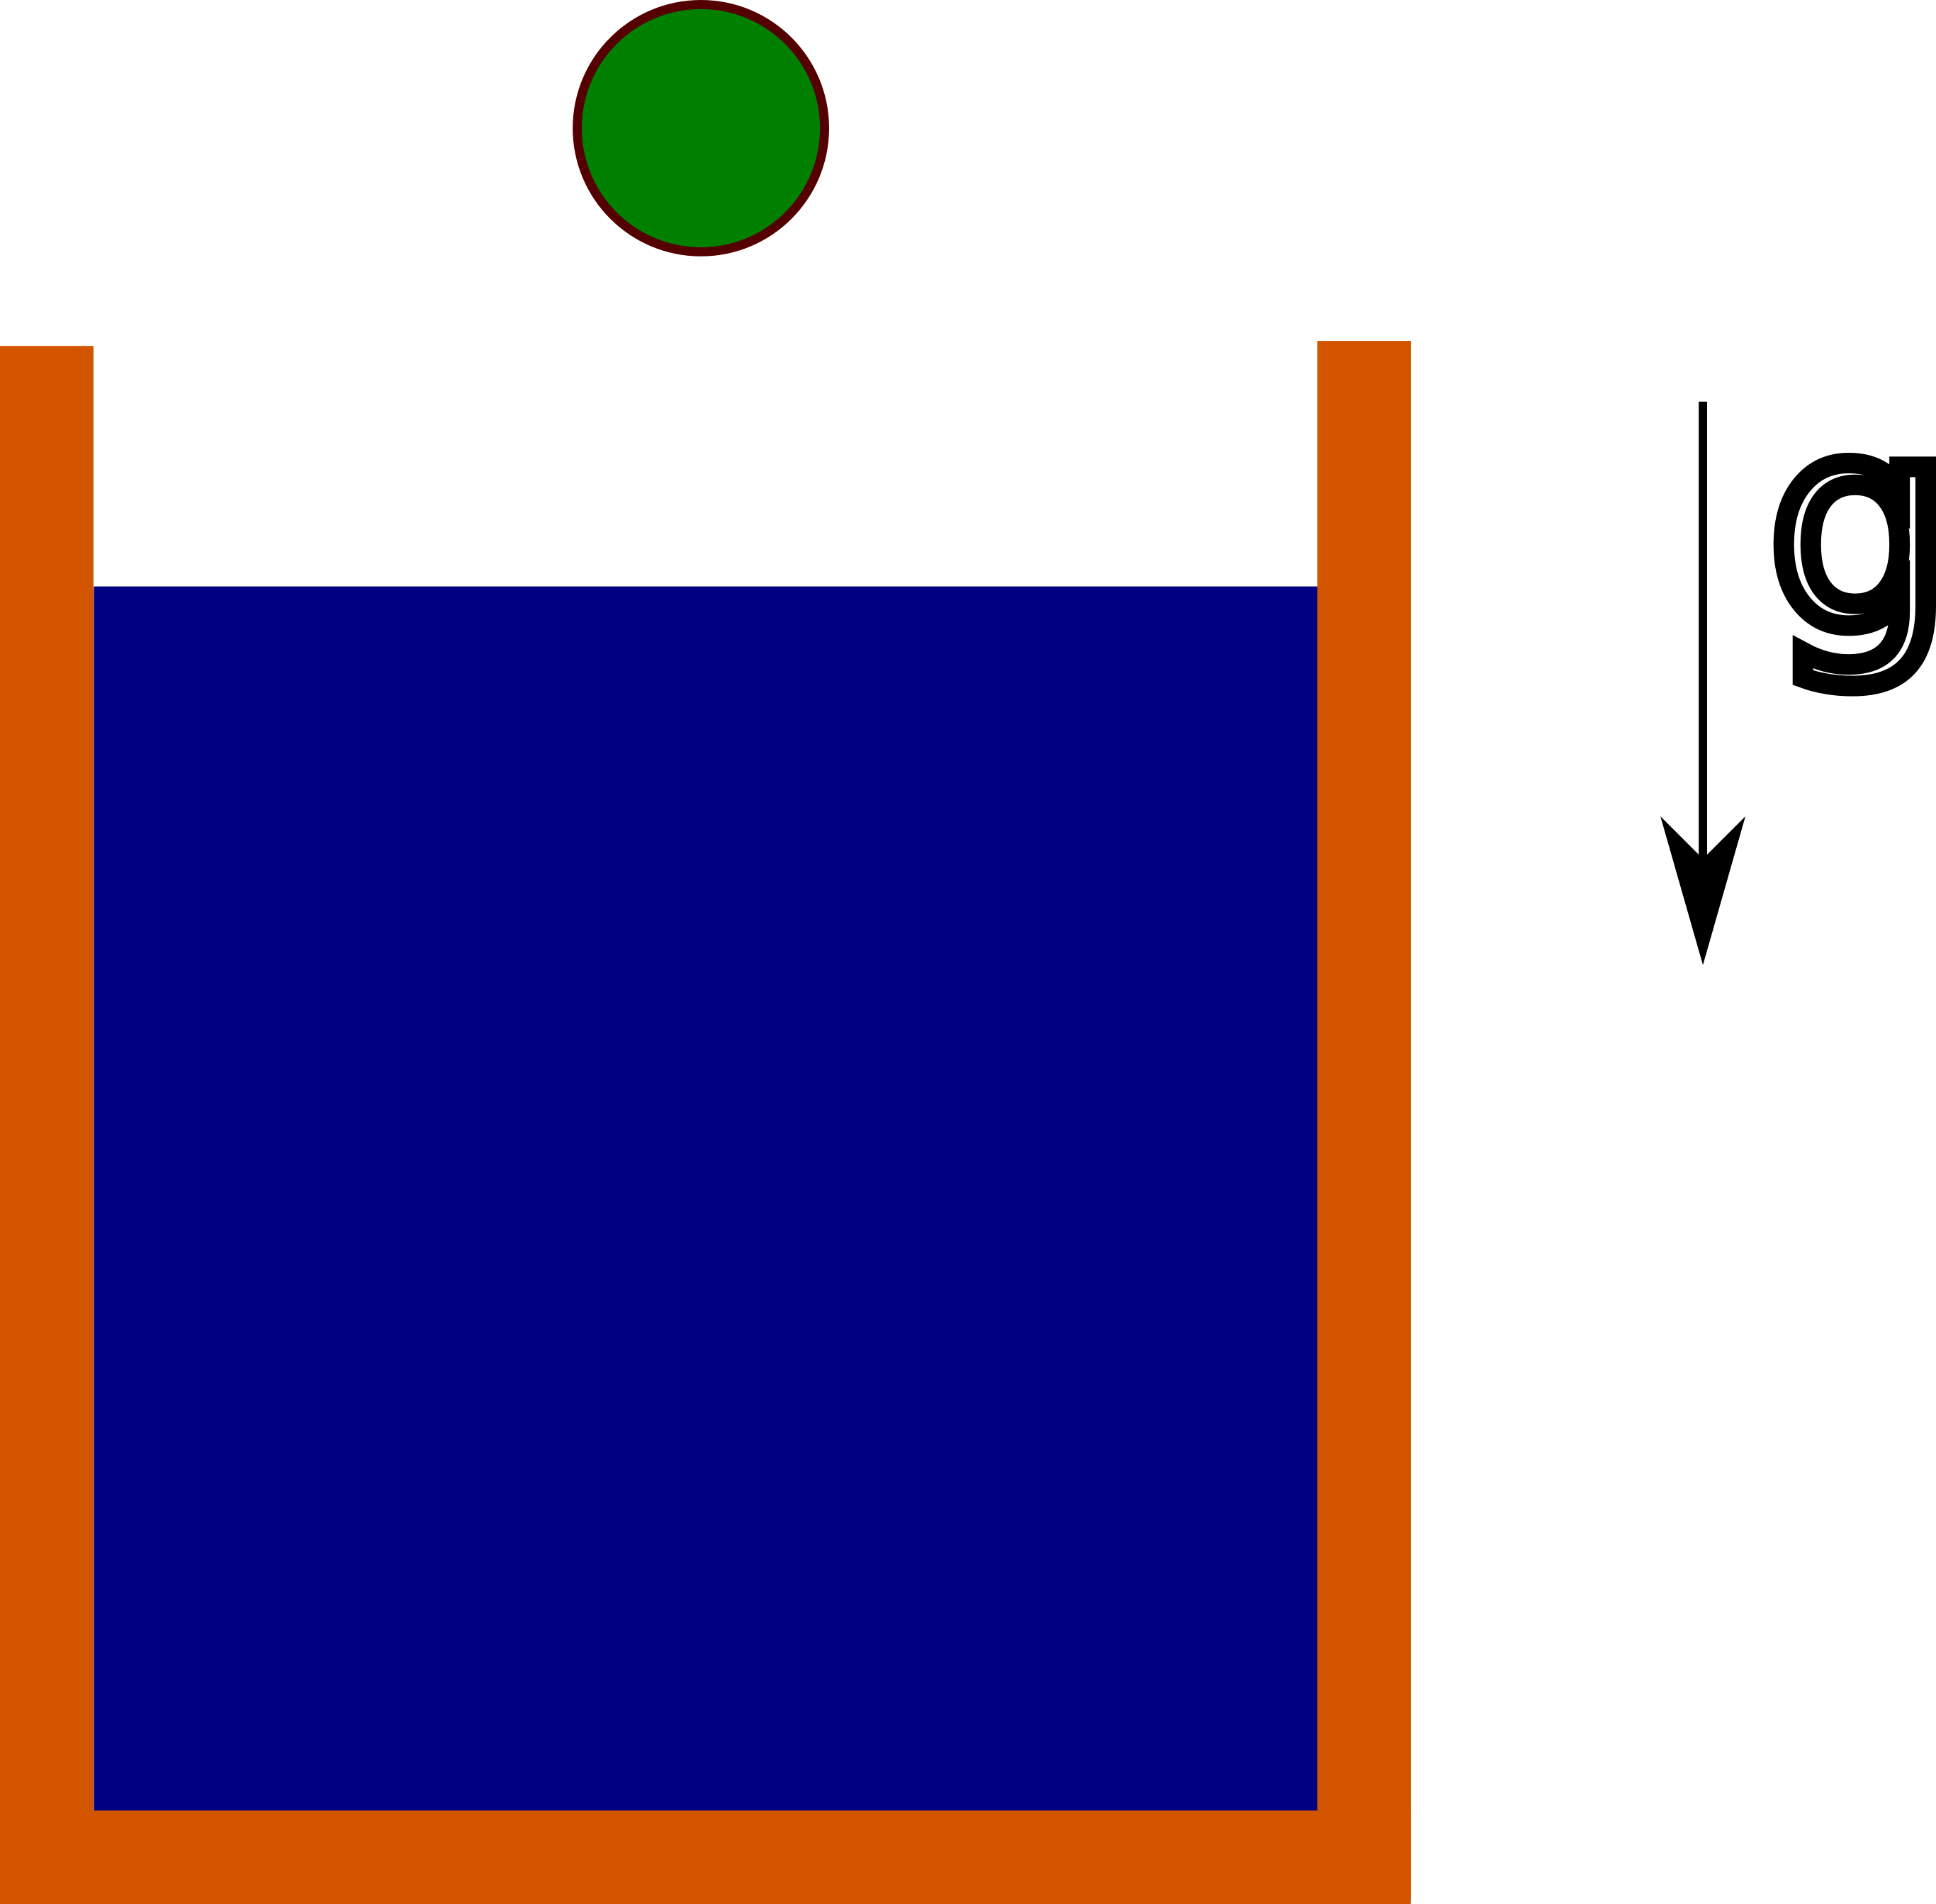
\includegraphics[width=0.4\textwidth]{images/rfc_01_skillen_2013_particle_entry_in_hs_tank/Skillen_2013_particle_entry_in_hs_tank}
  \caption{Half Buoyant}
  \label{fig:results_rfc_01_skillen_2013}
\end{figure}
To validate the rigid fluid coupling solver, we study the motion of a circular
cylinder dropping into a steady tank. This problem has been studied
experimentally by Greenhow and Lin
\citet{xxxx}. \Cref{fig:results_rfc_01_skillen_2013} shows the initial
configuration of the cylinder placed at $0.5$ m from the free surface. The
radius of the disc is taken as $0.11$ m, while we consider two cases with the
density of $500$ and $1000$ kg\,m\textsuperscript{-1}. The cylinder falls
under the gravity into the tank.

\todoin{Initial spacing, viscosity, gravity, h value, speed of sound, number of
  particles, resolution write in a table}

\cref{fig:result_rfc_01_result_displacement}, depicts the evolution of the
depth of penetration of the cylinder, compared against the experimental result
by \citet{xxxx}, numerical techniques of boundary element method
(BEM)(\cite{xxx}) and delta-plus SPH (\cite{xxx}). From
\cref{fig:result_rfc_01_result_displacement}, we find that the current solver
matches well with the experimental result and also converges while increasing
the resolution.
\begin{figure}[!htpb]
  \centering
  \begin{subfigure}{0.48\textwidth}
    \centering
    \includegraphics[width=1.0\textwidth]{figures/skillen_2013_water_entry_half_buoyant/penetration_vs_t}
    \subcaption{}%\label{fig:rings:ipst-nu-0.47-0}
  \end{subfigure}
  \begin{subfigure}{0.48\textwidth}
    \centering
    \includegraphics[width=1.0\textwidth]{figures/skillen_2013_water_entry_neutrally_buoyant/penetration_vs_t}
    \subcaption{}%\label{fig:rings:ipst-nu-0.47-1}
  \end{subfigure}
  \caption{}
\label{fig:result_rfc_01_result_displacement}
\end{figure}


\FloatBarrier%
\subsection{RFC validation 2: Two tandem particles entering into a tank}
\label{sec:rfc_validation_2_single_particle_entry}



\FloatBarrier%
\subsection{Mixing of spherical particles in a fluid tank}
\label{sec:mixing-spherical-particles-in-fluid-tank}



\FloatBarrier%
\subsection{Mixing of spherical particles of variable size in a fluid tank}
\label{sec:mixing-spherical-particles-in-fluid-tank}



\FloatBarrier%
\section{Conclusions}
\label{sec:conclusions}


% \section*{References}


\bibliographystyle{model6-num-names}
\bibliography{references}
\end{document}

% ============================
% Table template for reference
% ============================
% \begin{table}[!ht]
%   \centering
%   \begin{tabular}[!ht]{ll}
%     \toprule
%     Quantity & Values\\
%     \midrule
%     $L$, length of the domain & 1 m \\
%     Time of simulation & 2.5 s \\
%     $c_s$ & 10 m/s \\
%     $\rho_0$, reference density & 1 kg/m\textsuperscript{3} \\
%     Reynolds number & 200 \& 1000 \\
%     Resolution, $L/\Delta x_{\max} : L/\Delta x_{\min}$ & $[100:200]$ \& $[150:300]$\\
%     Smoothing length factor, $h/\Delta x$ & 1.0\\
%     \bottomrule
%   \end{tabular}
%   \caption{Parameters used for the Taylor-Green vortex problem.}%
%   \label{tab:tgv-params}
% \end{table}

%%% Local Variables:
%%% mode: latex
%%% TeX-master: "paper"
%%% fill-column: 78
%%% End:
